\chapter{Modelagem Preditiva por Aprendizado de Máquina}

\section{Coleta dos Dados}

Com o intuito de coletar os dados, foi desenvolvido um algoritmo de \textit{web scraping}, utilizando a biblioteca \textit{Beautiful Soup} da linguagem \textit{Python}. 
Essa biblioteca é amplamente empregada para extração e manipulação de informações a partir de páginas HTML e XML, permitindo a coleta automatizada e estruturada de grandes 
volumes de dados provenientes da web \cite{beautifulsoup}. O algoritmo implementado automatiza o acesso às páginas de estatísticas, realiza a extração das tabelas 
correspondentes a cada clube e temporada e armazena os dados de forma padronizada para posterior análise.

O site utilizado para a extração foi o FBref, uma ampla base de dados de estatísticas de futebol que disponibiliza dados detalhados de jogadores e equipes de diversas 
competições ao redor do mundo. O FBref se destaca por fornecer estatísticas avançadas, como gols esperados (xG), ações de pressão, passes progressivos e 
estatísticas defensivas, tornando-se uma fonte relevante para análises preditivas e modelagem estatística no contexto do futebol.

Com o objetivo de utilizar um volume de dados superior ao empregado por \textit{Baboota \& Kaur} (2018) e \textit{Joseph, Fenton \& Neil} (2006), bem como reduzir o 
risco de \textit{overfitting}, foram coletados os dados de todos os jogadores da \textit{Serie A} italiana e da \textit{Premier League} que atuaram ao longo de cinco 
temporadas (2019-2020, 2020-2021, 2021-2022, 2022-2023 e 2023-2024), além das tabelas de resultados de todos os jogos disputados nesse mesmo período.

A utilização de duas ligas distintas neste estudo possui o papel metodológico deevitar a ocorrência de \textit{data leakage} entre os conjuntos de 
treinamento, teste e validação dos modelos de AM. Para isso, os dados de uma liga são utilizados exclusivamente na etapa de treinamento, enquanto os 
dados da outra liga são reservados para teste e validação. Essa estratégia assegura que o modelo seja avaliado em um contexto completamente distinto daquele empregado no 
aprendizado, eliminando dependências estruturais entre amostras e proporcionando uma avaliação mais realista de sua capacidade de generalização.

Os dados obtidos foram armazenados no formato CSV, organizados em arquivos distintos para cada clube e temporada. Dessa forma, cada arquivo contém as estatísticas 
individuais dos jogadores de um determinado time em uma temporada específica, facilitando a organização, o pré-processamento e as etapas subsequentes da análise. 
Ao todo, foram coletados dados de 2900 jogadores pertencentes a 30 equipes da Serie A italiana e de 2399 jogadores pertencentes a 28 equipes da 
EPL. Assim, o conjunto de dados utilizado neste estudo totaliza 5299 registros de jogadores, distribuídos entre 58 equipes, 
que serviram de base para o desenvolvimento dos modelos preditivos.

\section{Pré-processamento dos Dados}

\subsection{Base de Dados dos Jogadores}

As tabelas extraídas do site FBref \cite{fbref} para todos os times e temporadas foram estruturadas de forma idêntica, contendo 47 atributos relacionados à idade, posição, minutos 
jogados, bem como estatísticas ofensivas (gols, assistências, passes decisivos, entre outras) e defensivas (bloqueios, desarmes, erros graves, entre outras) de cada 
jogador. Esses dados foram carregados em diferentes \textit{dataframes}, um para cada liga considerada, e posteriormente organizados por jogador, incluindo informações 
de clube, temporada e respectivos indicadores de desempenho. Ressalta-se que um mesmo atleta pode aparecer em diferentes temporadas e clubes dentro da organização 
adotada.

A Tabela~\ref{tab:features} apresenta a descrição completa das variáveis utilizadas no estudo.

\begingroup
\footnotesize
\renewcommand{\arraystretch}{1.15}

\begin{longtable}{>{\raggedright\arraybackslash}p{3.3cm} >{\raggedright\arraybackslash}p{10.7cm}}
\caption{Descrição das variáveis utilizadas no modelo}\label{tab:features}\\
\hline
\textbf{Variável} & \textbf{Descrição} \\
\hline
\endfirsthead

\hline
\textbf{Variável} & \textbf{Descrição} \\
\hline
\endhead

\multicolumn{2}{l}{\textbf{Identificação e contexto}}\\
Player & Nome do jogador. \\
Season & Temporada à qual os dados se referem. \\
Team & Clube pelo qual o jogador atuou na temporada. \\
Pos. & Posição principal do jogador em campo. \\
Idade & Idade do jogador durante a temporada. \\

\multicolumn{2}{l}{\textbf{Participação e minutagem}}\\
MP & Número de partidas disputadas. \\
Inícios & Número de partidas iniciadas como titular. \\
Min. & Total de minutos jogados. \\
90s & Minutos jogados convertidos em equivalentes de partidas completas (90 minutos). \\

\multicolumn{2}{l}{\textbf{Produção ofensiva (totais)}}\\
Gols & Número total de gols marcados. \\
Assis. & Número total de assistências realizadas. \\
G+A & Soma de gols e assistências. \\
G-PB & Gols marcados excluindo penalidades. \\
PB & Número de pênaltis convertidos. \\
PT & Número de pênaltis cobrados. \\

\multicolumn{2}{l}{\textbf{Disciplina}}\\
CrtsA & Cartões amarelos recebidos. \\
CrtV & Cartões vermelhos recebidos. \\

\multicolumn{2}{l}{\textbf{Métricas avançadas (totais)}}\\
xG & \textit{Expected Goals} (gols esperados), métrica que estima a probabilidade de finalizações resultarem em gol. \\
npxG & \textit{Expected Goals} excluindo penalidades. \\
xAG & \textit{Expected Assists} (assistências esperadas). \\
npxG+xAG & Soma de gols esperados sem pênaltis e assistências esperadas. \\

\multicolumn{2}{l}{\textbf{Progressão}}\\
PrgC & Corridas progressivas com a bola. \\
PrgP & Passes progressivos realizados. \\
PrgR & Recebimentos progressivos de passe. \\

\multicolumn{2}{l}{\textbf{Produção ofensiva (por 90 minutos)\textsuperscript{a}}}\\
Gols.1 & Gols por 90 minutos\textsuperscript{a}. \\
Assis..1 & Assistências por 90 minutos\textsuperscript{a}. \\
G+A.1 & Gols mais assistências por 90 minutos\textsuperscript{a}. \\
G-PB.1 & Gols sem pênaltis por 90 minutos\textsuperscript{a}. \\
G+A-PB & Gols mais assistências excluindo pênaltis por 90 minutos\textsuperscript{a}. \\
xG.1 & \textit{Expected Goals} por 90 minutos\textsuperscript{a}. \\
xAG.1 & \textit{Expected Assists} por 90 minutos\textsuperscript{a}. \\
xG+xAG & Soma de xG e xAG por 90 minutos\textsuperscript{a}. \\
npxG.1 & \textit{Expected Goals} sem pênaltis por 90 minutos\textsuperscript{a}. \\
npxG+xAG.1 & Soma de npxG e xAG por 90 minutos\textsuperscript{a}. \\

\multicolumn{2}{l}{\textbf{Ações defensivas}}\\
Div & Desarmes (\textit{tackles}) realizados. \\
TklW & Desarmes vencidos. \\
Terço Def & Desarmes realizados no terço defensivo do campo. \\
Terço Central & Desarmes realizados no terço central do campo. \\
Terço de Ataque & Desarmes realizados no terço ofensivo. \\
Div.1 & Tentativas de desarme. \\
Tent & Tentativas totais de desarme contra adversários. \\
Tkl\% & Percentual de sucesso nos desarmes. \\
Perdido & Número de vezes em que o jogador foi driblado. \\

\multicolumn{2}{l}{\textbf{Bloqueios e interceptações}}\\
Bloqueios & Número de ações de bloqueio (chutes ou passes bloqueados). \\
TC & Chutes bloqueados. \\
Passe & Passes bloqueados. \\
Crts & Interceptações realizadas. \\
Tkl+Int & Soma de desarmes e interceptações. \\
Def & Ações defensivas realizadas na área defensiva. \\
Erros & Erros que resultaram em finalizações adversárias. \\

\hline
\multicolumn{2}{l}{\footnotesize \textsuperscript{a} Variáveis normalizadas por 90 minutos (equivalente a uma partida completa).}\\
\multicolumn{2}{l}{\footnotesize Fonte: FBref (2026), adaptado pelo autor.}\\
\end{longtable}
\endgroup

Após a etapa de organização, os dados estruturados foram armazenados em um repositório público na plataforma GitHub, com o objetivo de garantir reprodutibilidade, 
transparência metodológica e facilidade de acesso para futuras análises. O repositório utilizado neste estudo está disponível em 
\url{https://github.com/LunusMax/epl-seriea-data}.

Em seguida, os \textit{dataframes} correspondentes a cada liga foram concatenados em um único conjunto, englobando todos os jogadores considerados no estudo, o qual foi 
utilizado nas etapas subsequentes da análise.

Considerando o elevado número de atributos e a possível correlação entre variáveis, foi aplicada uma técnica de redução de dimensionalidade com o objetivo de mitigar 
\textit{overfitting} e melhorar a eficiência computacional dos modelos de AM. Para isso, utilizou-se o Principal Component Analysis (PCA), conforme 
descrito na subseção a seguir.

\subsubsection{Principal Component Analysis (PCA)}

Para determinar o número ideal de componentes principais que a serem utilizados no PCA, foi gerado um \textit{Scree Plot}, conforme ilustrado na Figura~\ref{fig01}.

\begin{figure}[h]
    \centering
    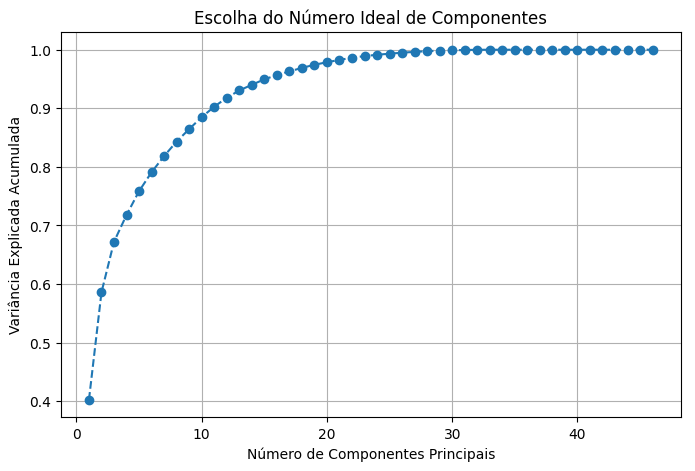
\includegraphics[width=1.0\linewidth]{imagens/pca_01.png}
    \caption{Escolha do Número Ideal de Componentes do PCA}
    {\small Fonte: do Autor, 2025}
    \label{fig01}
\end{figure}

O gráfico apresenta a variância explicada acumulada em função do número de componentes principais, permitindo identificar o ponto de inflexão, ou seja, o momento em que 
a adição de novos componentes passa a contribuir de forma marginal para a variância total dos dados. O eixo \textit{x} representa o número de componentes principais, 
enquanto o eixo \textit{y} exibe a variância explicada acumulada.

A partir da Figura~\ref{fig01}, observa-se que, acima de 20 componentes principais, o ganho de informação adicional se torna insignificante. 
Com base nessa análise, foram realizados testes com diferentes quantidades de componentes, garantindo que sempre eram utilizados no mínimo 20 componentes, 
de forma a preservar a maior quantidade possível de variância dos dados sem comprometer a eficiência do modelo. Optou-se, por fim, pela utilização de 
20 componentes principais, uma vez que esse valor já era suficiente para explicar 97,66\% da variância total dos dados, indicando que praticamente 
toda a informação relevante do conjunto original estava preservada nessa representação reduzida.

\subsection{Base de Dados dos Jogos}

Os dados dos jogos realizados entre as temporadas 2019-2020 e 2023-2024, obtidos na etapa de coleta, estavam organizados em 14 colunas. No entanto, 
grande parte dessas informações era irrelevante para a análise (por exemplo, horário e data das partidas, público, local e árbitro). 
Assim, para otimizar o conjunto de dados, foram removidos os atributos considerados ruído, mantendo-se apenas três elementos essenciais: time mandante, 
time visitante e resultado da partida.

A coluna de resultados foi transformada em valores numéricos por meio de um algoritmo em Python, em processo análogo a um \textit{encoder}: 
vitória do mandante foi codificada como '1', vitória do visitante como '2' e empate como '0'.

Com base nessa codificação, percorreu-se a base atribuindo três pontos a cada vitória e um ponto a cada empate. 
O resultado desse processamento foi uma tabela organizada por temporada, contendo cada clube e a respectiva pontuação acumulada.

\section{Treinamento do Modelo de AM}

Os dados de pontuação dos clubes foram organizados por temporada, enquanto as estatísticas individuais dos jogadores corresponderam sempre à temporada anterior. 
Dessa forma, o modelo utiliza informações conhecidas de desempenho prévio para estimar a pontuação final do clube na temporada subsequente. 
Adicionalmente, a pontuação dos clubes na temporada anterior foi incorporada como variável explicativa, de modo a capturar o histórico de desempenho recente da equipe.

O modelo de AM foi desenvolvido para prever a pontuação dos clubes ao longo das temporadas, com base no desempenho individual de seus jogadores. Para evitar 
vazamento de dados entre treinamento e teste, a base da Série A italiana foi utilizada no treinamento do modelo, enquanto a base da EPL foi destinada à etapa de teste.

\subsection{Modelo de Aprendizado de Máquina}

Para a etapa de previsão da pontuação dos clubes, foi implementado o modelo de MLP utilizando a biblioteca \textit{Keras}. O modelo foi construído 
no formato \textit{Sequential}, contendo três camadas densamente conectadas. A primeira camada recebe como entrada um vetor com dimensão igual ao 
número de atributos disponíveis, seguido por uma camada densa com 128 neurônios e função de ativação ReLU. Esta camada foi regularizada por meio de penalização L1, de 
forma a reduzir o risco de sobreajuste. 

Em seguida, aplicou-se normalização em lote (\textit{Batch Normalization}) e uma camada de \textit{Dropout} com taxa de 60\%, visando maior robustez e generalização. 
A segunda camada oculta é composta por 32 neurônios, também com ativação ReLU e regularização L1, seguida novamente por \textit{Batch Normalization} e \textit{Dropout} 
de 60\%. Por fim, a camada de saída é formada por um único neurônio linear, responsável por produzir a previsão da pontuação final do clube na temporada.

A arquitetura do modelo pode ser resumida da seguinte forma:

\begin{itemize}
    \item Camada de entrada: vetor de dimensão $n$ (atributos do jogador e do clube).
    \item Primeira camada oculta: \texttt{Dense(128)}, ativação ReLU, regularização L1.
    \item \texttt{Batch Normalization}.
    \item \texttt{Dropout(0.6)}.
    \item Segunda camada oculta: \texttt{Dense(32)}, ativação ReLU, regularização L1.
    \item \texttt{Batch Normalization}.
    \item \texttt{Dropout(0.6)}.
    \item Camada de saída: \texttt{Dense(1)}, ativação linear.
\end{itemize}
%%Essa configuração foi escolhida por equilibrar complexidade e capacidade de generalização, evitando sobreajuste em função do tamanho relativamente 
%%%limitado da base de dados.
O MLP foi escolhido como base para o modelo de previsão de pontuação no contexto do futebol por reunir propriedades teóricas e práticas que o tornam adequado para 
lidar com a natureza complexa e não linear dos dados esportivos. Entre as principais razões para essa escolha, destacam-se:

\begin{enumerate}
    \item \textbf{Capacidade de representação universal} —
    Um MLP com pelo menos uma camada oculta e funções de ativação não lineares é capaz de aproximar qualquer função mensurável \cite{Hornik1991}.
    No contexto do futebol, isso significa que o modelo pode aprender padrões não lineares entre variáveis de desempenho (como gols, desarmes, progressão). 
    Assim, o MLP não depende de hipóteses rígidas sobre a forma das relações entre variáveis, sendo capaz de aprendê-las diretamente dos dados.

    \item \textbf{Flexibilidade para entradas de alta dimensão} —
    De acordo com \textit{Goodfellow et. al., 2016}, cada camada de uma rede \textit{feedforward} aprende uma representação do vetor de entrada que torna 
    mais fácil a predição da saída desejada. 
    Essa característica confere ao MLP flexibilidade para lidar com conjuntos de dados de alta dimensionalidade, nos quais múltiplas variáveis interagem de forma não linear. 
    Mesmo com a aplicação prévia da técnica de \textit{Principal Component Analysis} (PCA), que reduz a dimensionalidade de 48 para 20 componentes principais, 
    o problema ainda envolve um espaço vetorial de considerável complexidade. 
    Nesse contexto, o MLP é capaz de explorar as relações não lineares entre os componentes principais, aprendendo representações 
    mais informativas que auxiliam na previsão de desempenho esportivo.

    \item \textbf{Treinamento eficiente via retropropagação} — 
    O algoritmo de \textit{backpropagation}, apresentado em \cite{Goodfellow2016}, permite o cálculo eficiente dos gradientes de erro e a atualização 
    simultânea dos pesos da rede por meio de gradiente descendente. 
    Isso viabiliza o treinamento em grandes bases de dados de futebol, reduz o tempo de convergência e possibilita otimizar métricas contínuas.
\end{enumerate}

Além dessas vantagens teóricas, o MLP oferece um equilíbrio entre capacidade de generalização, interpretabilidade e eficiência computacional, características 
desejáveis em modelos aplicados ao futebol, onde os dados são heterogêneos, ruidosos e interdependentes.

\begin{comment}
\section{Predição de Impacto de um Jogador}

Com o intuito de prever o impacto de jogadores no time, o algoritmo de AM

Em um primeiro momento, busca-se desenvolver um algoritmo capaz de predizer o impacto de um jogador em um time. Para essa tarefa, serão utilizadas três variáveis: 
\textit{team\_target}, \textit{season\_target} e \textit{player\_added}. O objetivo dessa abordagem é simular a busca de um time por um jogador antes do início da temporada, 
permitindo prever o impacto que ele terá ao longo da competição.

Conforme discutido por \textit{Baboota \& Kaur} (2018), a variável com maior influência na predição de resultados foi a forma recente do time. Seguindo esse princípio, 
serão aplicados pesos à forma do jogador, atribuindo maior relevância ao desempenho recente. Estatísticas mais antigas também serão consideradas, 
porém com um peso reduzido, garantindo que o modelo priorize informações mais atuais.

Com os dados preparados para análise, busca-se encontrar o melhor modelo de ML a partir de experimentação com diferentes algoritmos. O modelo base 
será selecionado a partir de métricas como o MAE (\textit{Mean Absolute Error}) e o $R^2$ \textit{score}.
\end{comment}